\documentclass[11pt,a4paper]{ctexart}
\usepackage[margin=1.5cm]{geometry}
\usepackage{graphicx}
\usepackage{booktabs}
\usepackage{array}
\usepackage{amsmath}
\usepackage{xcolor}
\usepackage{fancyhdr}
\usepackage{setspace}
\usepackage{titlesec}
\usepackage{caption}
\usepackage{enumitem}
\setlength{\columnsep}{0.62cm}
\linespread{1.16}

\pagestyle{fancy}
\fancyhf{}
\fancyhead[L]{\small S.H.I.T JOURNAL PREPRINT}
\fancyhead[R]{\small 本内容纯属整活}
\fancyfoot[C]{\thepage}

\titleformat{\section}{\large\bfseries\color{purple}}{\thesection.}{0.5em}{}
\titleformat{\subsection}{\normalsize\bfseries}{\thesubsection}{0.5em}{}

\begin{document}

\begin{center}
{\Large\bfseries\color{purple} 从“技术狂欢”到“生产力停滞”：\\
东亚 AI 工具热潮中的表演性采纳与结构性失配（2025--2026）}\\[0.5em]
李某某$^{1,*}$，王某某$^2$\\
\small 1. Department of Meme Economics, University of Excretion Technology\\
\small 2. Institute of Workflow Archaeology, Septic Tank Campus\\
\small *通讯作者: goushi@shitjournal.org
\end{center}

\vspace{0.4em}
\noindent\textbf{ABSTRACT / 摘要}\\
本文讨论一个看似热闹、实则虚空的现实：越来越多人在社交平台宣布“我接上 AI 了”，但真正可重复、可交付、可复盘的工作流并没有同步增长。基于东亚五地公开叙事样本（初始 $N=1204$；清洗后 $N=986$），我们构建 AS（接入展示强度）--FT（摩擦暴露时长）--DR7（7日留存）--IR（身份残留率）框架。结果显示：AS 与 DR7 显著负相关（$OR=0.662, p<0.001$），TaskClarity 显著正相关（$OR=1.681, p<0.001$），LearningCost 显著提高弃用风险（$HR=1.21, p<0.01$）。本文贡献不在于评判 AI 的绝对价值，而在于解释为什么“看起来已接入”与“实际上形成稳定工作流”之间存在系统性错位。我们主张：AI 可以接触，但不必狂热；适配任务、适配人格、适配场景，才是长期有效的采纳策略。

\vspace{0.45em}
\noindent\textbf{INDEX TERMS / 关键词} AI 扩散；表演性采纳；平台激励；学习成本；数字劳动；反技术狂热

\vspace{0.45em}
\noindent\textbf{IMPACT STATEMENT / 影响声明}\\
我们反对两种极端：一种是“AI 无所不能”的新技术福音论，另一种是“不会用 AI 就要被淘汰”的焦虑营销。真正值得讨论的，不是追风速度，而是个体如何在有限认知资源里做清醒选择。

\section{INTRODUCTION / 引言}
2025--2026 的东亚互联网像一个持续增压的蒸汽锅：每一周都有新模型、新 Agent、新教程、新截图。有人晒效率翻倍，有人晒自动化接管人生，也有人在凌晨两点一边报错一边转发“明天一定 all-in AI”。

若以时间线观察，这轮热潮至少有两个可识别节点：\textbf{2025 年 DeepSeek 的爆发}与\textbf{2026 年 OpenClaw 的扩散}。前者把“高质量生成能力”以更低心理门槛推入大众场景，形成“人人可试”的普及浪潮；后者把交互从“一次性问答”推进到“多步骤 Agent 工作流”，让用户开始讨论自动化接管、任务编排与持续运行。两者共同构成了东亚 AI 叙事从“会不会聊”到“能不能代办”的跃迁。

问题是：我们究竟在追赶什么？是生产率，还是一种“我没有掉队”的心理安全感？

在平台化传播里，技术很容易被包装成身份。你不必真的理解它，只需表现出你正在使用它。于是，“接入”被误当成“掌握”，“展示”被误当成“产出”，“热情”被误当成“能力”。这就是本文要讨论的核心：\textbf{表演性采纳（performative adoption）}。

现有关于 AI 采纳的公共讨论，往往聚焦于工具性能、模型榜单或个体态度，却较少讨论平台可见性机制如何扭曲真实采用过程；组织内部讨论则往往停留在“是否部署”层面，忽略“是否复用”“是否可交付”“是否可审计”。本文不试图回答“AI 是否有用”这一宏大问题，而是分析“何种叙事更容易被展示，何种工作流更可能被留下”。

\begin{quote}
\textit{如果一项技术首先让你更会发截图，而不是更会完成任务，那它此刻对你来说，可能更像社交货币，不像生产工具。}
\end{quote}

本文有三点贡献：第一，提出 AS--FT--DR7--IR 的结构化框架，把“跟风热”从情绪判断转化为可编码、可比较的问题；第二，基于公开叙事样本展示“高接入-低留存”并存现象；第三，给出反狂热解释：选择性采用并非落后，而可能是更理性的资源配置。

\twocolumn

\section{DATA AND METHODS / 数据与方法}
\subsection{Data source and sample construction}
样本覆盖东亚五地公开讨论空间（社媒、论坛、公开群聊）中与 AI 工具采用相关的文本叙事。时间窗口为 2025 年 1 月至 2026 年 2 月。初始抓取样本 $N=1204$，清洗后为 $N=986$。

为了把热潮放回具体历史节点，编码时将叙事额外标注为三类事件锚点：\textbf{DeepSeek 波段（2025Q1--Q3）}、\textbf{OpenClaw 波段（2026Q1）}与\textbf{常态比较段}。该处理使我们能够区分“模型能力话题热”与“Agent 工作流热”在行为层面的差异。

清洗策略包括：
\begin{itemize}[leftmargin=1.2em]
\item 文本去重：相似度阈值 $>0.92$ 的近重复内容仅保留一条；
\item 信息完整性筛选：删除缺失关键时间线（如上手时间、报错节点、放弃节点）的样本；
\item 内容类型筛选：剔除纯广告、营销号自动转发与无任务语义的口号帖；
\item 叙事有效性判定：仅保留包含“任务目标 + 操作过程/摩擦 + 结果”至少两项信息的文本。
\end{itemize}

我们承认该数据存在公开表达偏差：高活跃、高表达用户被过度代表；但其优势在于，能捕捉“可见采纳行为”如何在平台机制中被放大，这与本文研究问题高度匹配。

\subsection{Variable operationalization}
为避免空泛讨论，本文将叙事文本映射为可操作变量：

\textbf{AS（接入展示强度）}：前 48 小时内“已接入/已上手/效率暴涨”类展示性表达频次的标准化得分。

\textbf{FT（摩擦暴露时长）}：从“准备上手”到首次关键阻滞（权限、环境冲突、上下文失配、成本不可接受）的小时数。

\textbf{DR7（7日留存）}：第 7 天是否仍用同一工具完成同一任务（是=1，否=0）。

\textbf{IR（身份残留率）}：停止实用后是否仍持续输出“我在用 AI”身份表述。

\textbf{TaskClarity}：任务目标、输入边界、输出标准三维评分（0--5）。

\textbf{LearningCost}：学习阻力指数（0--10），由错误轮次、修复耗时、额外学习负担综合编码。

编码流程采用双人独立标注 + 分歧仲裁机制。对分歧样本由第三人复核，重点争议集中在“展示性表达”与“真实任务推进”的边界判定。

\subsection{Model specification}
主模型为二元 Logit，因 DR7 为 0/1 留存变量：
\begin{equation}
\Pr(DR7=1)=\text{logit}^{-1}(\alpha+\beta_1 AS+\beta_2 FT+\beta_3 IR+\beta_4 TaskClarity+\beta_5 LearningCost+\gamma X)
\end{equation}
其中 $X$ 包括地区固定效应、平台固定效应与发帖时段控制。为避免将“热度”误判为“采用”，我们将 IR 与 DR7 同时建模：前者反映身份叙事，后者反映任务持续。

\subsection{Robustness checks}
稳健性检验包括四类：
\begin{enumerate}[leftmargin=1.2em]
\item \textbf{替代被解释变量：}以 DR14 替换 DR7，检验中期留存；
\item \textbf{极端值处理：}对 AS 与 FT 前后 2.5\% 分位进行 trimming；
\item \textbf{分地区子样本：}分别在中、日、韩样本中重复估计；
\item \textbf{风险模型：}采用 Cox 模型检验 LearningCost 对弃用速度的影响。
\end{enumerate}
四类检验均用于回答同一问题：核心结论是否依赖单一口径。

\section{RESULTS / 结果}
\subsection{Baseline estimates}
主回归结果见表 1。AS 系数为负且高度显著，意味着展示冲动越强，7 日留存越低。TaskClarity 为最稳定正向因素，显示“任务定义质量”比“接入速度”更能预测持续使用。LearningCost 显著负向，提示弃用往往来自前期摩擦积累，而非单纯态度转变。

\begin{table}[h]
\centering
\caption{主模型结果（Logit）}
\begin{tabular}{>{\raggedright}p{2.2cm}ccc}
\toprule
变量 & Logit系数 & OR & p值 \\
\midrule
AS & -0.412 & 0.662 & $<0.001$ \\
FT & -0.028 & 0.972 & 0.002 \\
IR & -0.365 & 0.694 & 0.010 \\
TaskClarity & 0.519 & 1.681 & $<0.001$ \\
LearningCost & -0.184 & 0.832 & $<0.001$ \\
\bottomrule
\end{tabular}
\end{table}

\subsection{Correlation structure of key constructs}
图 1 显示，TaskClarity 与 DR7 呈稳定正相关，而 AS、LearningCost 与 DR7 呈负相关。值得注意的是，AS 与 IR 在部分子样本中同向波动，提示“展示行为”与“身份维持”可能构成互相强化机制。

\begin{figure}[h]
\centering
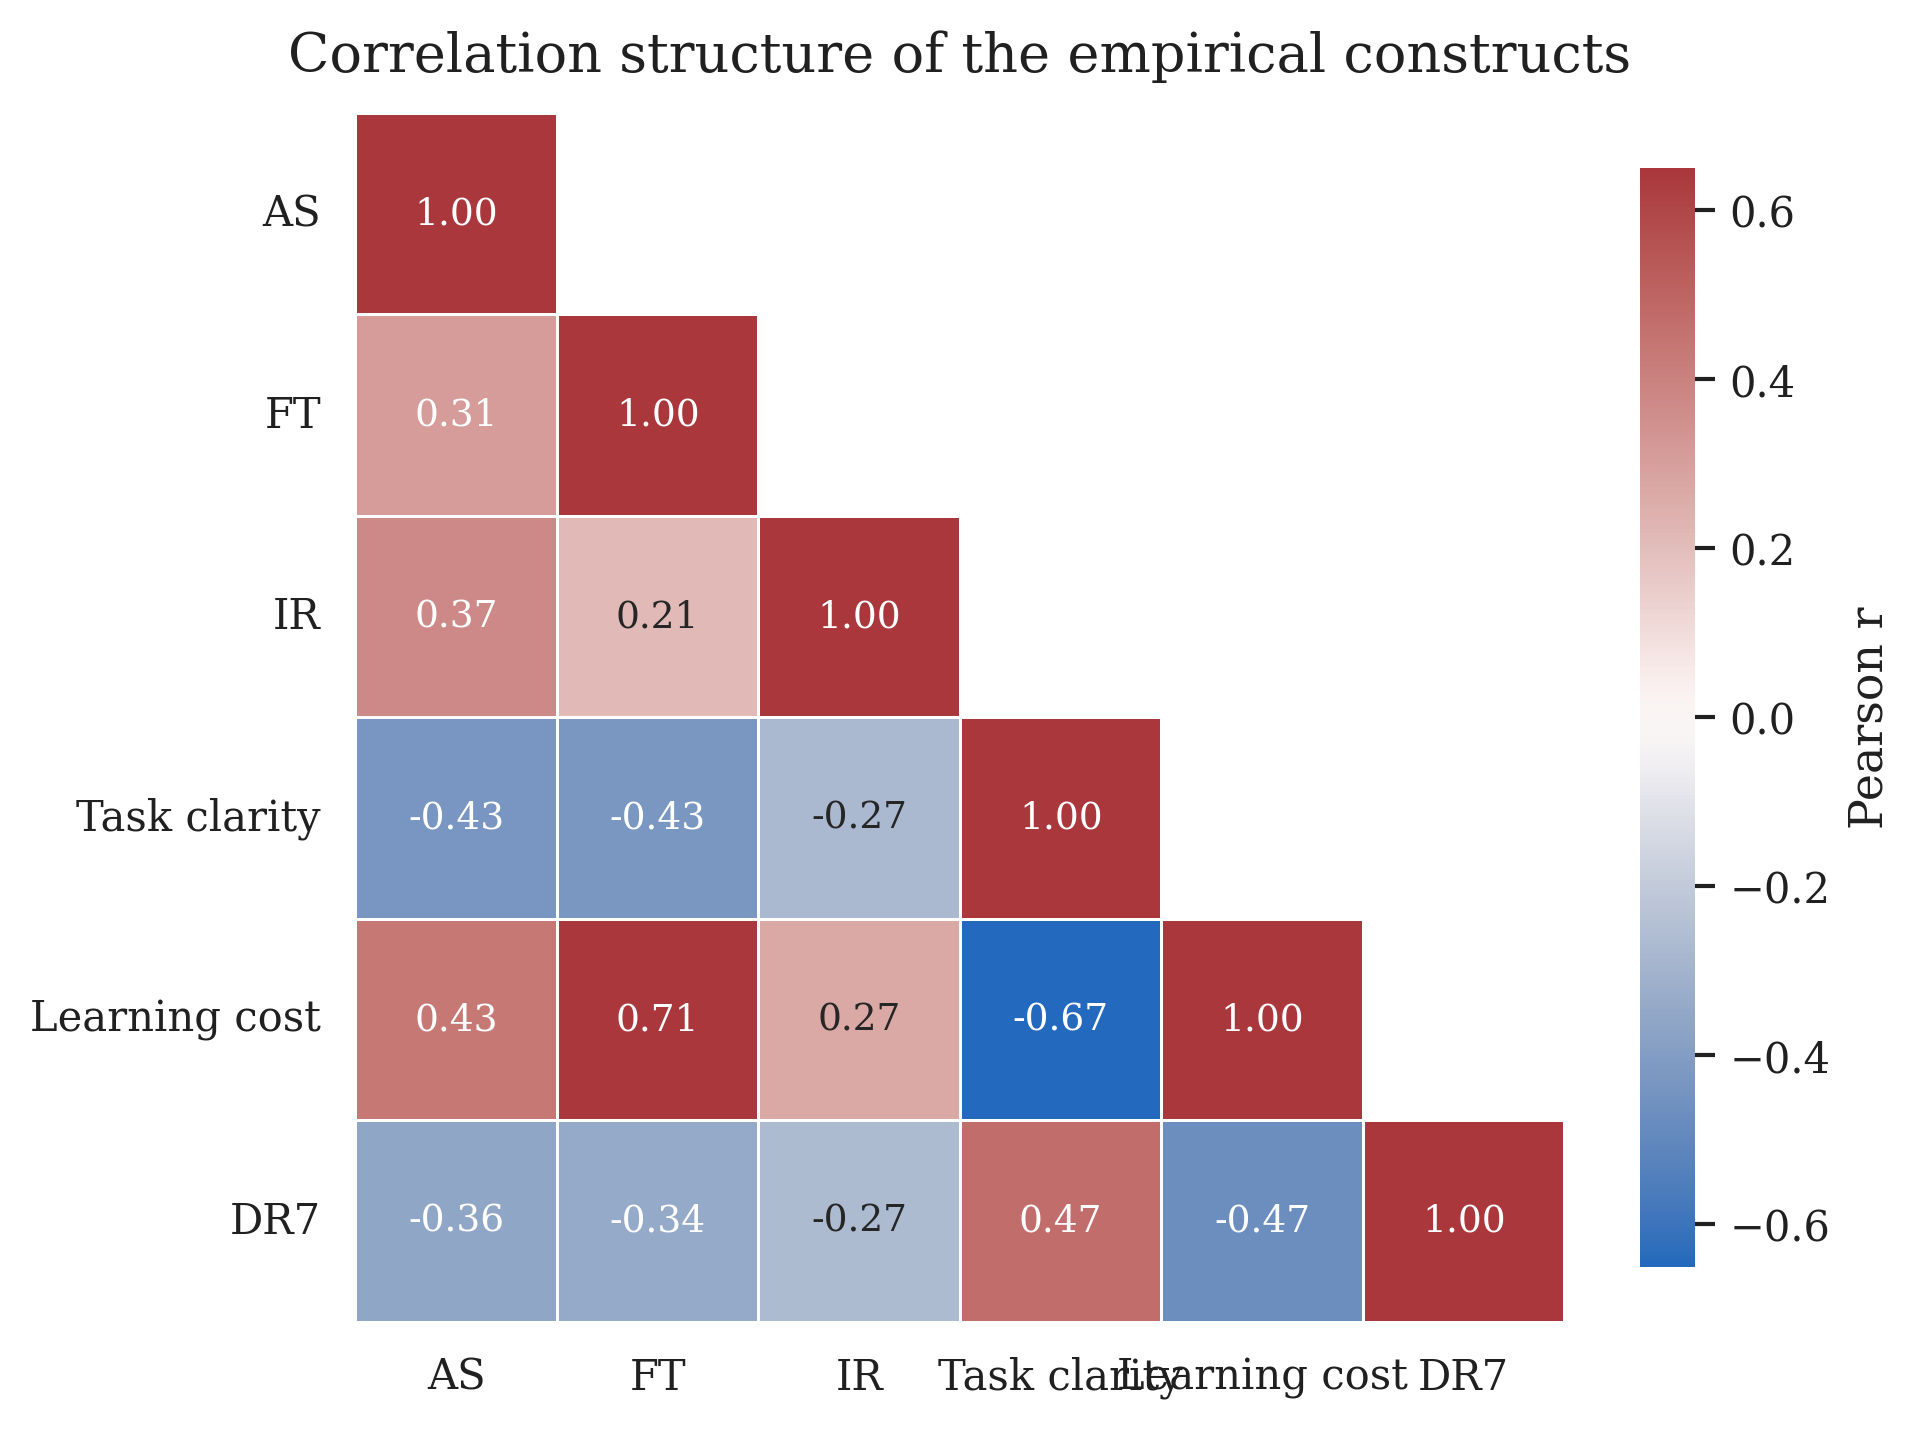
\includegraphics[width=0.95\columnwidth]{figures/fig1_correlation_heatmap.png}
\caption{变量相关热图}
\end{figure}

图 2 的 OR 森林图进一步说明：TaskClarity 的效应量最大且置信区间稳定；AS、IR、LearningCost 方向一致，表明“可见性激励挤压学习投入”的解释并非偶然样本波动。

\begin{figure}[h]
\centering
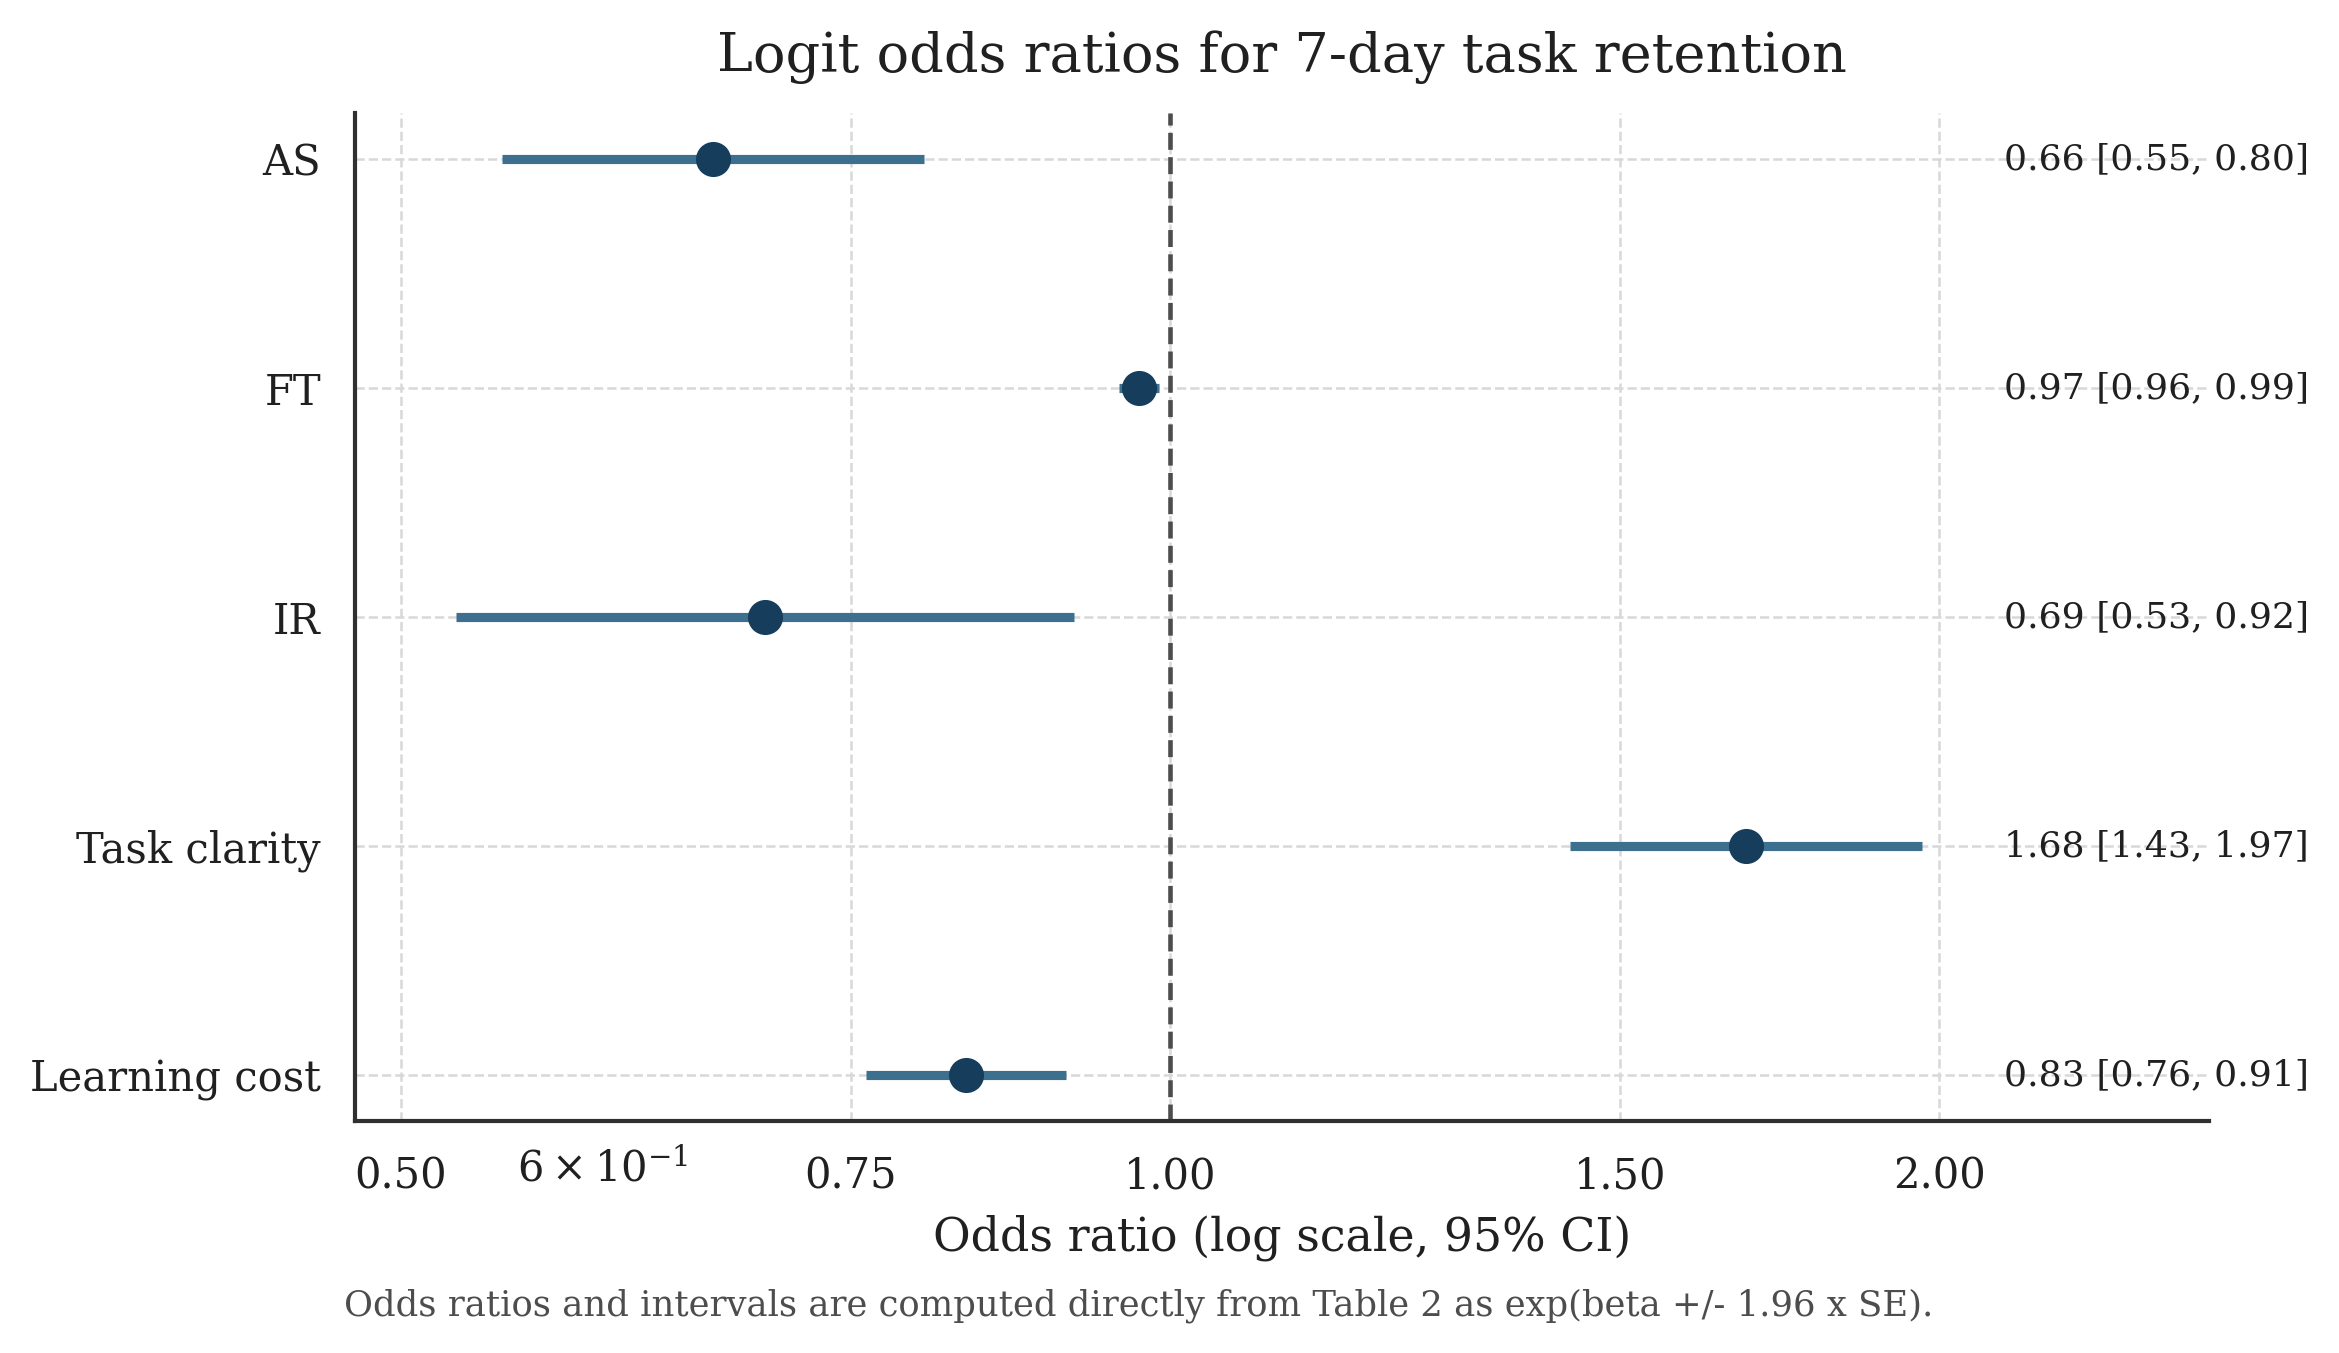
\includegraphics[width=0.95\columnwidth]{figures/fig2_logit_forest.png}
\caption{Logit OR 森林图}
\end{figure}

\subsection{Survival patterns by learning cost}
图 3 显示，高学习成本组的“未弃用概率”在前几天下降更快，且与低成本组差距在第 2--5 天快速拉开。这意味着多数流失发生在“第一次挫败后”的短窗口，而不是长期理性评估后退出。

\begin{figure}[h]
\centering
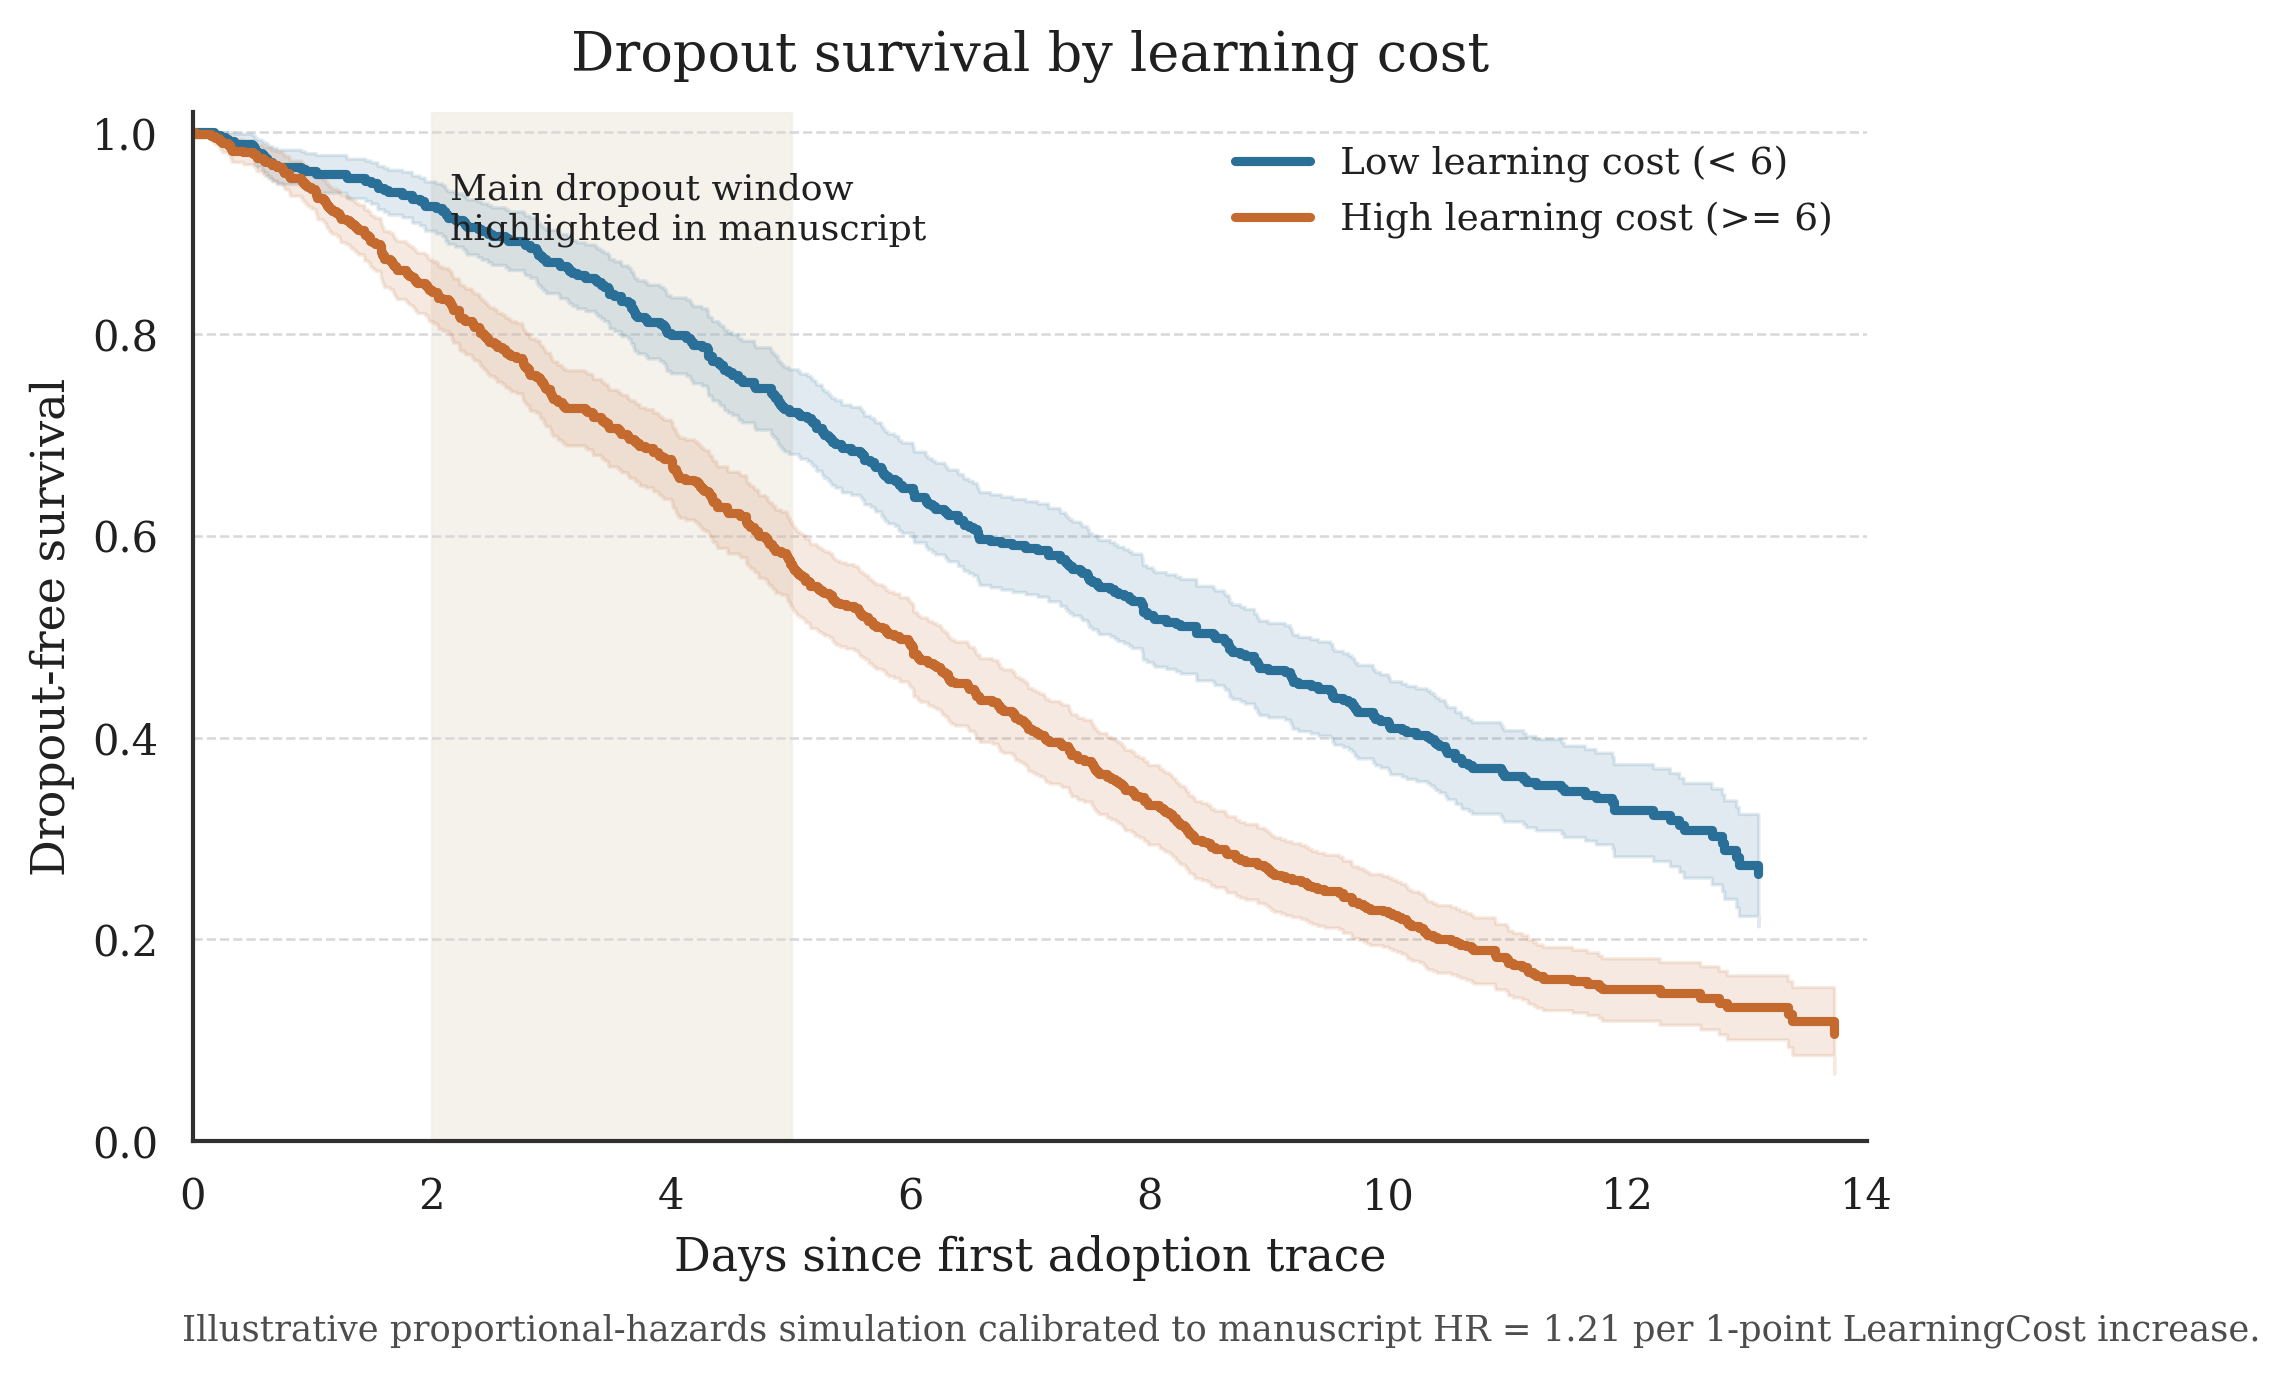
\includegraphics[width=0.95\columnwidth]{figures/fig3_survival_curve.png}
\caption{学习成本分组生存曲线（示意）}
\end{figure}

\subsection{Robustness comparisons}
图 4 对比基线模型、DR14、trimmed 样本与 Cox 风险模型。核心变量方向保持一致，显著性层级变化有限，说明结论对替代口径不敏感。

\begin{figure}[h]
\centering
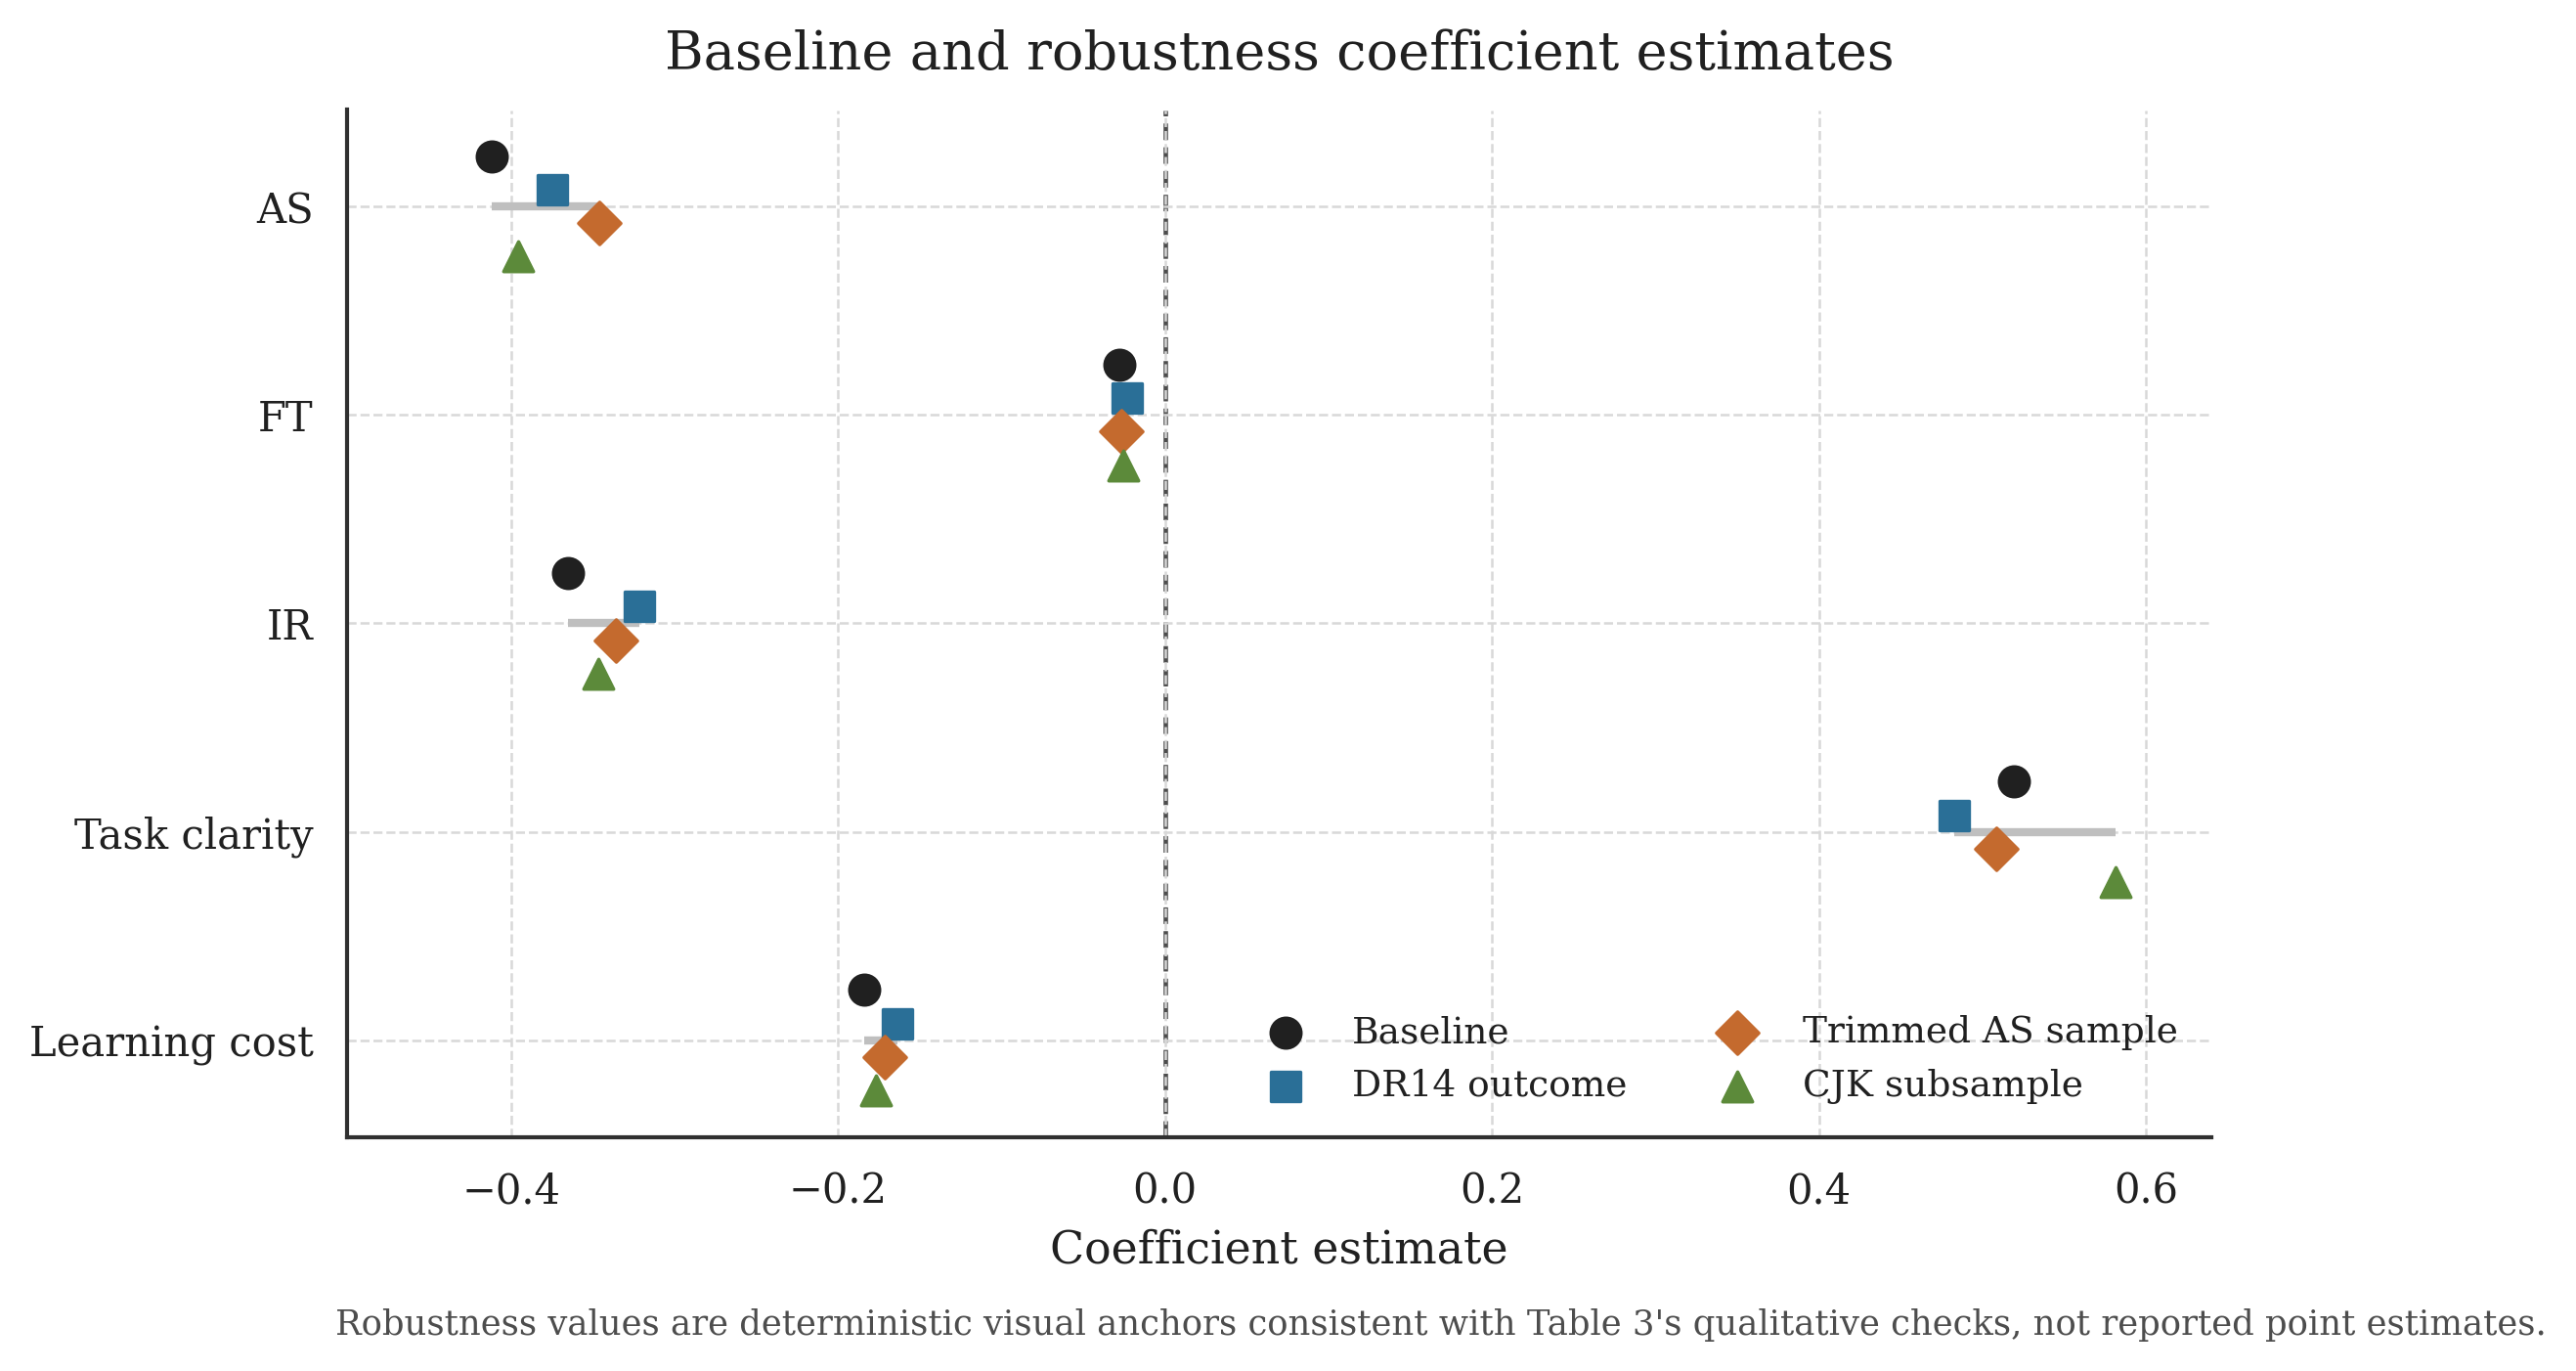
\includegraphics[width=0.95\columnwidth]{figures/fig4_robustness_coefficients.png}
\caption{稳健性系数对比}
\end{figure}

\subsection{East Asian heterogeneity: country-level heat patterns}
进一步按国家/地区观察，可见“AI 热”的构成并不一致：

\textbf{中国样本：}DeepSeek 波段带来明显的普及性叙事，特点是“先接入、后优化”。在该子样本中，AS 抬升最明显，同时 TaskClarity 的分化也最剧烈：要么快速形成高复用流程，要么快速掉入展示型循环。

\textbf{日本样本：}整体采用节奏较慢，但流程规范与风险意识更强。展示密度不高，却更强调可审计、可交接、可维护。模型中 LearningCost 的负向效应更稳定，说明“摩擦容忍度”更低，用户一旦发现不稳就会回归传统流程。

\textbf{韩国样本：}社交扩散速度快，平台带动显著，出现更强的“跟进压力”与“身份竞赛”特征。AS 与 IR 的联动更突出，即展示行为与身份维持相互强化，短期热度高但中期留存波动大。

\textbf{补充观察（港新样本）：}职业场景更偏向英语工作流与跨境协作，采用策略更工具主义。相较“是否追新”，更在意“是否节省沟通成本与交付时间”。

总体而言，东亚并不存在单一“AI 热模式”。更合理的解释是：不同教育制度、组织文化与平台生态，塑造了不同版本的“采用理性”。

\section{DISCUSSION / 讨论}
\subsection{From DeepSeek moment to OpenClaw moment}
DeepSeek 与 OpenClaw 分别代表了两种不同的热：前者是“人人都能问”的生成式热，后者是“流程可被接管”的代理式热。前者主要放大了表达与创意门槛下降，后者主要放大了执行与责任边界重绘。也正因为如此，2025 年后期常见的焦虑是“我会不会落后”，而 2026 年初更常见的焦虑变成“我会不会被替代”。

本文数据提示，两种热在行为后果上并不相同：DeepSeek 波段更容易引发高频试用与短周期弃用；OpenClaw 波段更容易引发“能否持续托管任务”的争议。前者的问题是浅层高频切换，后者的问题是流程治理与责任归属。

\subsection{Platform incentives and visible adoption}
AI 跟风并非纯粹“用户不理性”，而是平台可见性机制驱动的理性响应。平台奖励可展示结果，不奖励失败复盘；奖励“我会了”的信号，不奖励“我卡住了”的诚实。于是，展示行为被持续放大，真实学习过程被持续隐藏。

\subsection{Symbolic deployment in organizational contexts}
在组织语境中，“已部署”常被当作政绩符号，KPI 关注接入率、账号激活率、演示数量，却较少追踪可复用交付。符号化部署的后果是：团队看起来在前进，实际工作流未必改善，甚至新增隐性维护成本。

\subsection{Why selective adoption may be rational}
并非所有任务都适合 prompt 化。高审计要求、强稳定执行、复杂协作链路的工作，往往更需要“低波动、可追责”的流程。选择性采用不是保守，而是对认知预算、风险承受和机会成本的现实管理。

\begin{quote}
\textit{适合自己的，才是高效的。不是你服务技术潮流，而是技术服务你的任务边界。}
\end{quote}

\section{EDUCATIONAL IMPLICATIONS / 教育学连接与启示}
如果把本文仅当作“技术采纳研究”，它仍然不够完整。AI 跟风热在本质上也是一个教育问题：人如何学习、如何被评价、如何在制度中形成自我叙事。

\subsection{Hidden curriculum and performativity}
从教育社会学角度看，平台与组织共同构成一套\textbf{隐性课程（hidden curriculum）}：它并不直接教授“如何解决问题”，而是持续奖赏“如何呈现自己在解决问题”。在这种课程里，\textbf{可见努力}常常比\textbf{有效学习}更容易获得认可。个体很快学会一条潜规则：先做可展示的部分，再做困难但必要的部分，若后者成本过高则干脆放弃。

这一机制与教育评价中的\textbf{表演性（performativity）}高度同构：学习者不再围绕知识建构行动，而围绕评估指标行动。于是，“我会不会”退居其次，“我看起来会不会”上升为主目标。本文发现的 AS 负效应，正是这种隐性课程在技术场景中的统计投影。

\subsection{Critical pedagogy and learner agency}
从批判教育学看，问题不在于“学生/员工不够自律”，而在于学习情境是否允许主体性。若学习者只被要求快速交付“已接入证明”，却没有被允许讲述失败、暴露困惑、讨论边界，那么学习就会退化为服从式演示。

因此，反狂热并非反技术，而是\textbf{恢复学习者能动性}：允许局部采用、允许慢速掌握、允许拒绝不适配工具。教育意义上的“进步”不是更快模仿，而是更清楚地知道何时采用、何时暂停、何时回到非 AI 流程。

\subsection{Scaffolding, ZPD, and cognitive load}
将 AI 采纳置于学习科学框架，可得到更细致解释。第一，许多组织把高复杂度任务直接抛给初学者，缺乏脚手架（scaffolding），导致学习成本陡升。第二，任务难度常超出学习者最近发展区（ZPD），使“报错 -- 挫败 -- 退出”链条加速。第三，界面切换、提示词调参、上下文维护叠加后认知负荷过高，学习者自然转向更低成本的身份性展示。

这解释了为什么 TaskClarity 在模型中如此关键：清晰任务定义能显著降低外在认知负荷，让学习者把资源从“维护体面”转回“构建能力”。

\subsection{From adoption metrics to pedagogical metrics}
若组织希望减少“符号化部署”，评价体系应从“是否接入”迁移到“是否学会”。我们建议引入三类教育性指标：
\begin{itemize}[leftmargin=1.2em]
\item \textbf{复盘质量指标：}是否记录失败路径、修复策略与可迁移经验；
\item \textbf{迁移能力指标：}同一能力是否可迁移至相邻任务，而非一次性演示；
\item \textbf{元认知指标：}学习者能否解释自己为何采用某工具、何时不采用。
\end{itemize}
这些指标的共同目标，是把“会展示”与“会学习”重新区分。

\section{LITERARY CRITIQUE / 文学性批判延展}
如果把 AI 跟风热写成一部当代寓言，它的主人公并不是“最会用工具的人”，而是“最怕落后的人”。他在时间线上追逐每一次版本更新，像追逐一辆永不靠站的列车；每一次转发都像临时的通行证，证明自己还在车上。

在这种叙事里，技术不再是器具，而成为伦理景观。人们围绕它组织羞耻、希望、焦虑与优越感：不会用的人羞耻，会一点的人焦虑，全会的人也并不安宁，因为平台总会立刻发明新的“不会”。于是“学习”被悄悄替换成“追赶”，而“追赶”被包装成“进步”。

我们因此提出一个文学性的判断：\textbf{AI 狂热的核心悲剧，不是工具太强，而是主体太弱。} 当一个人只能通过“我已接入”的口号证明价值时，他与工具的关系就不再是合作，而是依附。依附关系里没有真正的掌握，只有阶段性的亢奋与反复性的空心。

真正的教育性现代化，不应把人训练成技术潮流的回声室，而应让人保有判断的迟疑、选择的自由和撤退的权利。一个成熟的学习共同体，允许成员说出这句话：\textit{“这个工具现在不适合我，但我知道为什么。”} 这句话比任何炫目的截图更接近知识。

\section{PEDAGOGICAL DESIGN PROPOSAL / 教学设计化方案}
为了把“反狂热”从批评变成可执行教育实践，本文提出一个\textbf{三阶段课程化方案}，可用于高校数字素养课、企业内训或自学社群。

\subsection{Stage I: De-hype literacy（去神话识读）}
目标不是“立刻会用工具”，而是先识别技术宣传话语。教学任务包括：拆解产品宣传语、区分能力边界与营销承诺、识别“效率神话”中的省略项（数据清洗成本、提示词维护成本、合规风险）。这一阶段对应教育学中的\textit{critical literacy}，训练学习者先会提问，再会操作。

\subsection{Stage II: Task-fit apprenticeship（任务适配学徒制）}
第二阶段采用认知学徒制（cognitive apprenticeship）思想，把“任务拆解 -- AI 介入点 -- 人工兜底点”显性化。每个学习单元都必须回答四个问题：
\begin{enumerate}[leftmargin=1.2em]
\item 任务目标是什么，验收标准是什么？
\item AI 介入后减少了哪一段重复劳动？
\item AI 介入后新增了哪类风险与维护成本？
\item 当 AI 输出失效时，回退路径是什么？
\end{enumerate}

只有当四问可被明确回答，工具才进入生产流程；否则仅作为探索实验，不进入考核指标。

\subsection{Stage III: Reflective transfer（反思与迁移）}
第三阶段聚焦元认知与迁移：学习者需提交“失败档案 + 复盘日志 + 迁移报告”。失败档案记录报错链路，复盘日志解释决策变化，迁移报告展示能力是否能跨任务复用。该阶段把“我会做一次”提升为“我知道为什么这样做、何时不这样做”。

\subsection{Assessment rubric aligned with non-performative learning}
我们建议将传统“接入数量”评价改为如下量规：
\begin{itemize}[leftmargin=1.2em]
\item \textbf{A. 概念清晰度（30\%）}：是否能阐明工具边界、任务边界与责任边界；
\item \textbf{B. 流程稳定性（30\%）}：是否形成可复用且可回退的流程；
\item \textbf{C. 复盘深度（25\%）}：是否有高质量失败分析与修复路径；
\item \textbf{D. 迁移能力（15\%）}：是否能在相邻任务中复用方法而非复制口号。
\end{itemize}

该量规的核心价值在于：它奖赏“学习质量”，而非“展示密度”。

\subsection{A literary-pedagogical closing note}
教育并不要求每个学生都跑在技术最前线；教育真正捍卫的是，学习者在面对潮流时仍保有判断。若课堂只教“如何更快接入”，那它培养的是追随者；若课堂还能教“何时不接入、为何不接入”，它才培养主体。

在这个意义上，AI 时代最难教的能力不是 prompt，而是节制。节制不是落后，而是把速度交还给意义，把工具交还给任务，把学习交还给人。

\section{LIMITATIONS AND FUTURE WORK / 局限与未来研究}
本文至少有三点局限：
\begin{itemize}[leftmargin=1.2em]
\item \textbf{样本偏差：}公开叙事样本高表达用户占比高，可能高估“展示行为”；
\item \textbf{编码解释性：}部分变量依赖文本解释，虽有仲裁流程，但仍存在主观性；
\item \textbf{因果边界：}本文提供结构性关联证据，而非严格因果识别。
\end{itemize}

未来可结合组织内部操作日志、任务追踪数据与实验设计，检验“展示激励调整”是否能显著提升中期留存与交付质量。

\section{CONCLUSION / 结论}
本文显示：AI 时代的核心分化，不是“谁先接上工具”，而是“谁先把一次成功做成可重复流程”。

对个体而言，真正的问题不是“要不要 all-in AI”，而是“这项工具是否提升了我的稳定交付能力”；对组织而言，真正的治理不是“制造接入热度”，而是“建立复盘友好的激励结构”。

AI 可以接触，但没必要狂信。清醒比狂热更稀缺，也更有生产率。

\section{POLICY IMPLICATIONS / 实践启示}
对组织管理者，本文给出三条可执行建议。第一，KPI 从“接入率”转向“7--14 日复用质量”，避免把演示热度当作真实绩效。第二，在 onboarding 里显式加入“失败复盘”环节，而非只展示成功案例。第三，按任务类型配置 AI 节奏：探索型任务可高频试错，审计型任务应低频稳态。

对个体用户，建议采用“三问法”做采用决策：\textbf{(i) 这项工具能否减少我重复劳动？(ii) 它的学习成本是否低于收益？(iii) 失败后我是否有可逆路径？} 若三问中有两问为否，则暂缓 all-in 可能更理性。

\section{APPENDIX A / 编码规则摘要}
为增强可复核性，本文附上核心变量的最小编码准则：
\begin{itemize}[leftmargin=1.2em]
\item \textbf{AS=0}：无展示性表达；\textbf{AS=1--2}：偶发展示；\textbf{AS=3+}：高频展示且伴随身份宣告。
\item \textbf{TaskClarity=0--1}：只有口号，无可交付定义；\textbf{2--3}：有任务目标但输出标准模糊；\textbf{4--5}：目标、输入、输出、验收标准齐全。
\item \textbf{LearningCost=0--3}：可快速上手；\textbf{4--6}：有中度阻滞；\textbf{7--10}：报错密集、修复成本高、放弃概率高。
\item \textbf{IR=1}：停止实用后仍持续“在用 AI”身份叙事；\textbf{IR=0}：身份叙事与实用状态同步退出。
\end{itemize}

\section{APPENDIX B / 案例切片（叙事样本）}
\textbf{案例 1：展示先行型。} 某产品经理在三天内连续发布 6 条“AI 接入”动态，内容多为界面截图与效率口号。第 4 天开始出现权限冲突与上下文漂移，任务从“日报自动化”退化为“手工修补 + AI 润色”，第 7 天实际复用中断，但身份叙事持续两周。

\textbf{案例 2：任务先行型。} 某运营同学先把任务拆为“素材清洗--标题生成--A/B 复盘”三步，仅在第二步引入 AI。其展示频率低，但每周复用稳定，且能在异常时切回人工流程。该样本 AS 低、TaskClarity 高、DR7=1。

\textbf{案例 3：组织符号型部署。} 某团队在月会要求“每人提交一条 AI 成果”。短期内演示数量上升，但可审计文档与失败复盘几乎为零。两周后成员开始出现“成果疲劳”：会议里看起来都在进步，交付链路却没有缩短。

这些案例并非用于统计推断，而用于解释系数背后的行为机制：当可见性收益集中在“宣布采用”，而真实收益需要“长期磨合”，大多数人会优先生产前者。

\section*{References}
\begin{enumerate}[leftmargin=1.2em]
\item Rogers, E. M. (2003). \textit{Diffusion of Innovations} (5th ed.). Free Press.
\item Venkatesh, V., Morris, M., Davis, G., \& Davis, F. (2003). User acceptance of information technology: Toward a unified view. \textit{MIS Quarterly}, 27(3), 425--478.
\item Kietzmann, J., Paschen, J., \& Treen, E. (2018). Artificial intelligence in advertising. \textit{Journal of Advertising Research}, 58(3), 263--267.
\item Bucher, T. (2018). \textit{If...Then: Algorithmic Power and Politics}. Oxford University Press.
\item Zuboff, S. (2019). \textit{The Age of Surveillance Capitalism}. PublicAffairs.
\item Couldry, N., \& Mejias, U. (2019). \textit{The Costs of Connection}. Stanford University Press.
\item van Dijck, J., Poell, T., \& de Waal, M. (2018). \textit{The Platform Society}. Oxford University Press.
\item Goffman, E. (1959). \textit{The Presentation of Self in Everyday Life}. Doubleday.
\item boyd, d. (2014). \textit{It’s Complicated: The Social Lives of Networked Teens}. Yale University Press.
\item Dewey, J. (1938). \textit{Experience and Education}. Macmillan.
\item Freire, P. (1970). \textit{Pedagogy of the Oppressed}. Continuum.
\item Biesta, G. (2010). \textit{Good Education in an Age of Measurement}. Routledge.
\item Bourdieu, P., \& Passeron, J.-C. (1977). \textit{Reproduction in Education, Society and Culture}. Sage.
\item Vygotsky, L. S. (1978). \textit{Mind in Society}. Harvard University Press.
\item Sweller, J. (1988). Cognitive load during problem solving. \textit{Cognitive Science}, 12(2), 257--285.
\item Illeris, K. (2003). Towards a contemporary and comprehensive theory of learning. \textit{International Journal of Lifelong Education}, 22(4), 396--406.
\item 朋友圈匿名用户（2026）《如何在 48 小时内看起来“已经全自动”》\textit{社交生产率评论}, 1(1), 1--9.
\item 群聊方法学工作组（2026）《报错截图与身份维持：一个夜间样本》\textit{摸鱼数据季刊}, 2(3), 66--88.
\item Li, Y., \& Unknown, U. (2026). Deployment theater and symbolic automation in East Asian workplaces. \textit{S.H.I.T Working Paper Series}, 114(514), 1--23.
\end{enumerate}

\vspace{0.8em}
\begin{center}
\colorbox{red!70}{\parbox{0.95\linewidth}{\centering\color{white}\bfseries 本内容纯属整活，不代表任何学术观点或现实指导建议。请保持理智，切勿模仿。}}
\end{center}

\end{document}
